\definecolor{plantucolor0000}{RGB}{254,254,206}
\definecolor{plantucolor0001}{RGB}{168,0,54}
\definecolor{plantucolor0002}{RGB}{180,167,229}
\definecolor{plantucolor0003}{RGB}{0,0,0}
\definecolor{plantucolor0004}{RGB}{173,209,178}

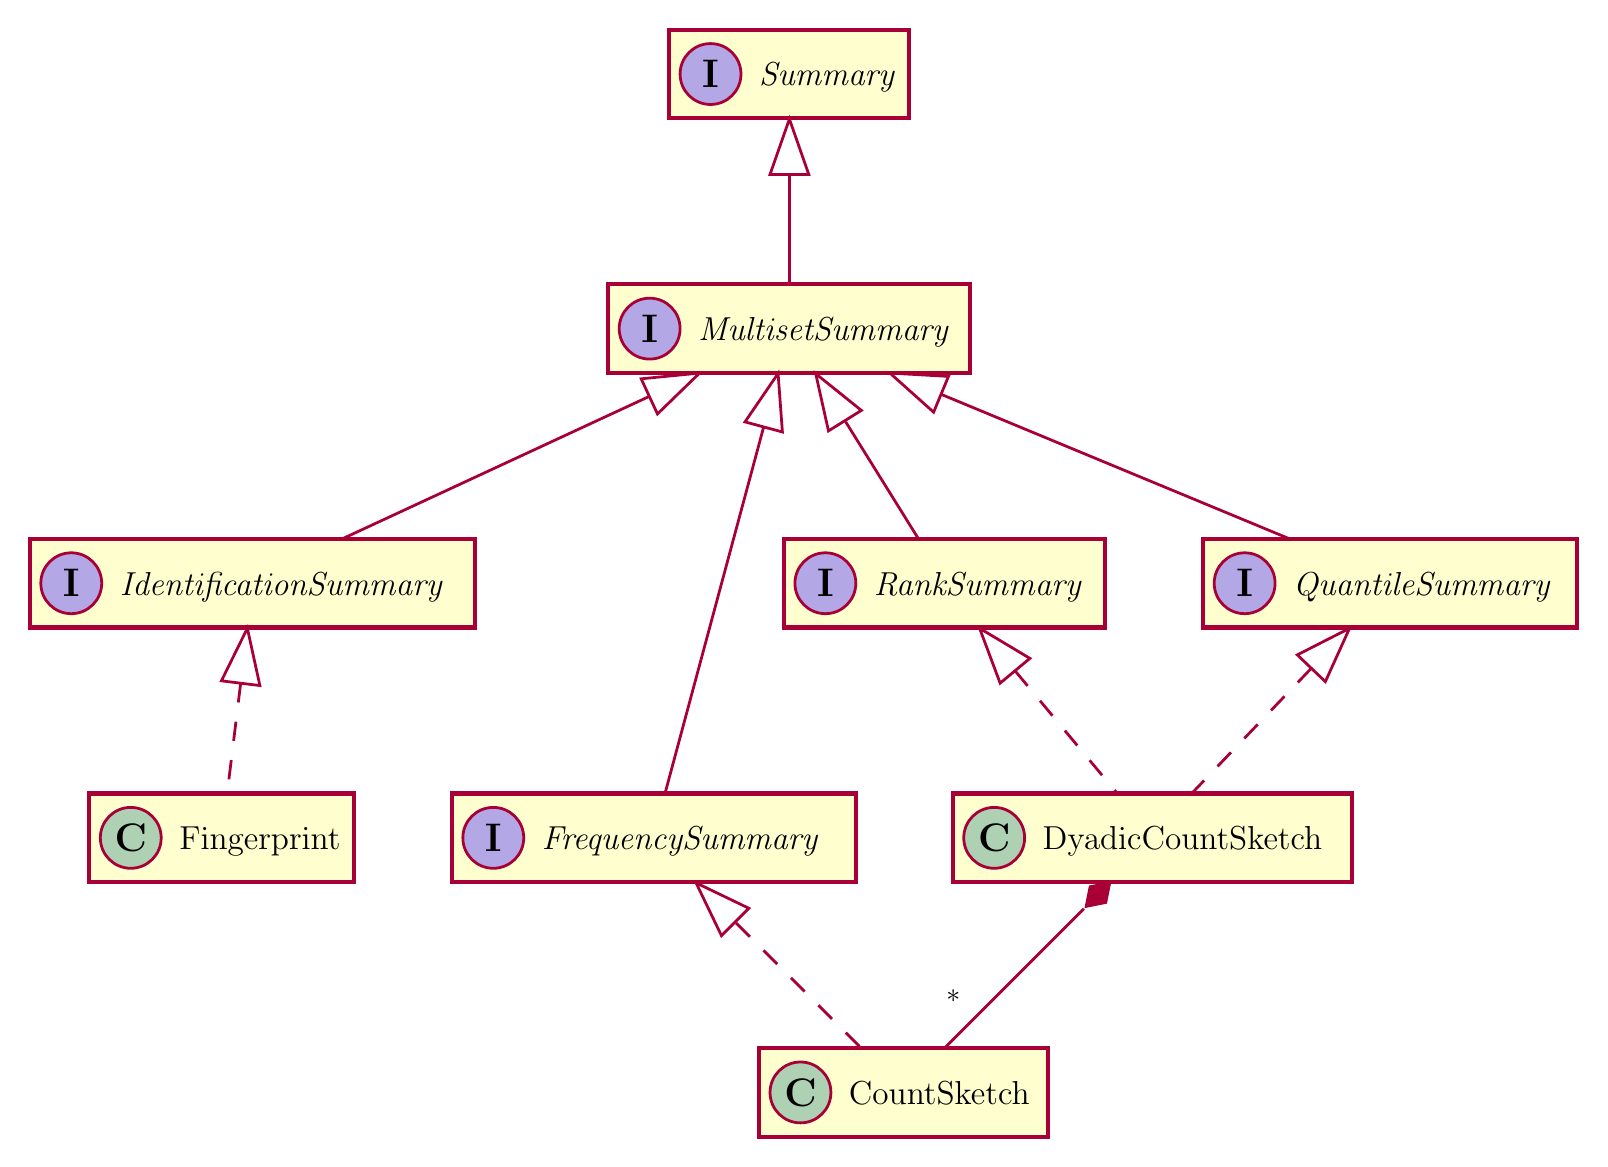
\begin{tikzpicture}[
  yscale = -1,
  pstyle0/.style = {color=plantucolor0001,fill=plantucolor0000,line width=1.5pt},
  pstyle1/.style = {color=plantucolor0001,fill=plantucolor0002,line width=1.0pt},
  pstyle2/.style = {color=plantucolor0001,fill=plantucolor0004,line width=1.0pt},
  pstyle3/.style = {color=plantucolor0001,line width=1.0pt},
  pstyle4/.style = {color=plantucolor0001,line width=1.0pt,dash pattern=on 7.0pt off 7.0pt},
]
  \draw[pstyle0] (238pt,7pt) rectangle (324.7652pt,39pt);
  \draw[pstyle1] (253pt,23pt) ellipse (11pt and 11pt);
  \node at (253pt,23pt)[]{\textbf{\Large I}};
  \node at (267pt,15.3945pt)[below right,color=black]{\textit{\large Summary}};
  \draw[pstyle0] (216pt,99pt) rectangle (346.8pt,131pt);
  \draw[pstyle1] (231pt,115pt) ellipse (11pt and 11pt);
  \node at (231pt,115pt)[]{\textbf{\Large I}};
  \node at (245pt,107.3945pt)[below right,color=black]{\textit{\large MultisetSummary}};
  \draw[pstyle0] (7pt,191pt) rectangle (167.9704pt,223pt);
  \draw[pstyle1] (22pt,207pt) ellipse (11pt and 11pt);
  \node at (22pt,207pt)[]{\textbf{\Large I}};
  \node at (36pt,199.3945pt)[below right,color=black]{\textit{\large IdentificationSummary}};
  \draw[pstyle0] (159.5pt,283pt) rectangle (305.5333pt,315pt);
  \draw[pstyle1] (174.5pt,299pt) ellipse (11pt and 11pt);
  \node at (174.5pt,299pt)[]{\textbf{\Large I}};
  \node at (188.5pt,291.3945pt)[below right,color=black]{\textit{\large FrequencySummary}};
  \draw[pstyle0] (279.5pt,191pt) rectangle (395.5732pt,223pt);
  \draw[pstyle1] (294.5pt,207pt) ellipse (11pt and 11pt);
  \node at (294.5pt,207pt)[]{\textbf{\Large I}};
  \node at (308.5pt,199.3945pt)[below right,color=black]{\textit{\large RankSummary}};
  \draw[pstyle0] (431pt,191pt) rectangle (566.2046pt,223pt);
  \draw[pstyle1] (446pt,207pt) ellipse (11pt and 11pt);
  \node at (446pt,207pt)[]{\textbf{\Large I}};
  \node at (460pt,199.3945pt)[below right,color=black]{\textit{\large QuantileSummary}};
  \draw[pstyle0] (28.5pt,283pt) rectangle (124.263pt,315pt);
  \draw[pstyle2] (43.5pt,299pt) ellipse (11pt and 11pt);
  \node at (43.5pt,299pt)[]{\textbf{\Large C}};
  \node at (57.5pt,291.3945pt)[below right,color=black]{\large Fingerprint};
  \draw[pstyle0] (270.5pt,375pt) rectangle (374.9645pt,407pt);
  \draw[pstyle2] (285.5pt,391pt) ellipse (11pt and 11pt);
  \node at (285.5pt,391pt)[]{\textbf{\Large C}};
  \node at (299.5pt,383.3945pt)[below right,color=black]{\large CountSketch};
  \draw[pstyle0] (340.5pt,283pt) rectangle (484.9412pt,315pt);
  \draw[pstyle2] (355.5pt,299pt) ellipse (11pt and 11pt);
  \node at (355.5pt,299pt)[]{\textbf{\Large C}};
  \node at (369.5pt,291.3945pt)[below right,color=black]{\large DyadicCountSketch};
  \draw[pstyle3] (281.5pt,59.61pt) ..controls (281.5pt,73.31pt) and (281.5pt,88.22pt) .. (281.5pt,98.96pt);
  \draw[pstyle3] (274.5pt,59.27pt) -- (281.5pt,39.27pt) -- (288.5pt,59.27pt) -- (274.5pt,59.27pt) -- cycle;
  \draw[pstyle3] (230.83pt,139.51pt) ..controls (195.84pt,155.74pt) and (150.33pt,176.85pt) .. (120.08pt,190.89pt);
  \draw[pstyle3] (227.94pt,133.13pt) -- (249.03pt,131.06pt) -- (233.83pt,145.83pt) -- (227.94pt,133.13pt) -- cycle;
  \draw[pstyle3] (272.13pt,150.79pt) ..controls (261.4pt,190.66pt) and (244.29pt,254.19pt) .. (236.55pt,282.97pt);
  \draw[pstyle3] (265.45pt,148.7pt) -- (277.41pt,131.2pt) -- (278.97pt,152.34pt) -- (265.45pt,148.7pt) -- cycle;
  \draw[pstyle3] (301.83pt,148.67pt) ..controls (310.83pt,163.13pt) and (320.98pt,179.44pt) .. (328.14pt,190.96pt);
  \draw[pstyle3] (295.62pt,151.95pt) -- (291pt,131.27pt) -- (307.51pt,144.55pt) -- (295.62pt,151.95pt) -- cycle;
  \draw[pstyle3] (336.55pt,138.83pt) ..controls (375.9pt,155.15pt) and (427.75pt,176.66pt) .. (462.06pt,190.89pt);
  \draw[pstyle3] (333.61pt,145.19pt) -- (317.82pt,131.06pt) -- (338.98pt,132.26pt) -- (333.61pt,145.19pt) -- cycle;
  \draw[pstyle4] (83.21pt,243.12pt) ..controls (81.52pt,256.95pt) and (79.67pt,272.09pt) .. (78.34pt,282.96pt);
  \draw[pstyle3] (76.26pt,242.27pt) -- (85.63pt,223.27pt) -- (90.16pt,243.97pt) -- (76.26pt,242.27pt) -- cycle;
  \draw[pstyle4] (262.27pt,329.77pt) ..controls (277.41pt,344.91pt) and (295.17pt,362.67pt) .. (307.46pt,374.96pt);
  \draw[pstyle3] (256.96pt,334.36pt) -- (247.77pt,315.27pt) -- (266.86pt,324.46pt) -- (256.96pt,334.36pt) -- cycle;
  \draw[pstyle4] (363.11pt,238.73pt) ..controls (375.55pt,253.66pt) and (389.94pt,270.93pt) .. (399.97pt,282.96pt);
  \draw[pstyle3] (357.65pt,243.11pt) -- (350.22pt,223.27pt) -- (368.4pt,234.15pt) -- (357.65pt,243.11pt) -- cycle;
  \draw[pstyle4] (470.06pt,237.77pt) ..controls (455.58pt,252.91pt) and (438.62pt,270.67pt) .. (426.87pt,282.96pt);
  \draw[pstyle3] (465.03pt,232.89pt) -- (483.91pt,223.27pt) -- (475.16pt,242.56pt) -- (465.03pt,232.89pt) -- cycle;
  \draw[pstyle3] (387.88pt,324.62pt) ..controls (371.77pt,340.73pt) and (351.26pt,361.24pt) .. (337.54pt,374.96pt);
  \draw[color=plantucolor0001,fill=plantucolor0001,line width=1.0pt] (397.23pt,315.27pt) -- (390.1589pt,316.6842pt) -- (388.7447pt,323.7553pt) -- (395.8158pt,322.3411pt) -- (397.23pt,315.27pt) -- cycle;
  \node at (334.716pt,350.481pt)[below right,color=black]{*};
\end{tikzpicture}
